% Requiere en main.tex: \usepackage{float}, \usepackage{graphicx}, \usepackage{url} (o hyperref)

\section{Desarrollo}

Tenemos como objetivo realizar una búsqueda de información mediante Inteligencia de Fuentes Abiertas (OSINT) para encontrar la mayor cantidad de datos posibles sobre dos agentes de la UNAM, documentando los aspectos relevantes de su identidad y rutinas. Todo se hizo únicamente con fuentes públicas, con fines didácticos y sin contactar a los agentes.

Partimos del hecho de que conocemos los alias de los agentes (Miri y Chipotles), así como sus nombres completos (Miriam Torres Bucio y Gerardo Emiliano Figueroa Sandoval), información obtenida fácilmente a partir de los registros públicos de la UNAM y de los medios de contacto de nuestro grupo de clase, al ser figuras académicas asignadas a nuestro curso.

%==========================================================
\subsection{Investigación: Agente Miri}

Comenzamos por investigar a la primera agente, Miri. Para ello, realizamos una búsqueda en Google con su nombre completo, usando comillas para forzar la coincidencia exacta de la cadena, es decir, buscamos \texttt{"Miriam Torres Bucio"}. De primeras obtuvimos resultados en portales profesionales como LinkedIn y en el directorio de la Facultad de Ciencias de la UNAM.

\begin{figure}[H]
    \centering
    
\includegraphics[width=0.6\textwidth]{Imagenes/Busqueda1.png}
    \caption{Búsqueda en Google.}
\end{figure}

Los motores de búsqueda convencionales no arrojaron más datos, así que la investigación se centró en buscar manualmente en los buscadores internos de distintas redes sociales. Pusimos su nombre completo y lo fuimos dividiendo en partes, combinando apellidos y nombres, hasta encontrar coincidencias. De esta forma encontramos un Facebook personal que parece ser de ella y, al comparar las fotos de perfil con las de sus otras cuentas, pudimos confirmar que se trataba de la misma persona. Cabe mencionar que el alias del enlace de Facebook (\texttt{mimy.torres.3}) sugiere que usa ``Mimy'' como apodo.

\subsubsection{Perfil Profesional y Académico}
\begin{itemize}
    \item \textbf{Actividad en la UNAM:} Se desempeña como Ayudante de profesor, de jornada parcial, en el área de Ciencias de la Computación desde el año 2023, según su perfil de LinkedIn.
    \item \textbf{Ubicación declarada:} Ciudad de México, México.
    \item \textbf{Aptitudes:} Python y SQL, ambas asociadas a su puesto de ayudante.
    \item \textbf{Correo institucional:} \texttt{miriamt@ciencias.unam.mx}
    \item \textbf{Red profesional:} Su LinkedIn muestra apenas 1 contacto y 1 seguidor, y no tiene publicaciones recientes, por lo que su huella profesional en esa red es muy discreta.
    \item \textbf{Intereses profesionales:} Sigue a las empresas Busco Junior (plataforma orientada a perfiles junior) y VASS (consultora tecnológica). Como inferencia, esto sugiere interés en entrar al mercado laboral de TI, aunque no es un dato confirmado.
\end{itemize}

\subsubsection{Huella Digital y Redes Sociales}
A través del mapeo de su presencia digital, se identificaron los siguientes perfiles públicos:
\begin{itemize}
    \item \textbf{LinkedIn:} \url{https://www.linkedin.com/in/miriam-torres-bucio-959960300/}
    \item \textbf{Facebook:} \url{https://www.facebook.com/mimy.torres.3}
    \item \textbf{GitHub:} \url{https://github.com/TorresMiriam}
\end{itemize}

\begin{figure}[H]
    \centering
    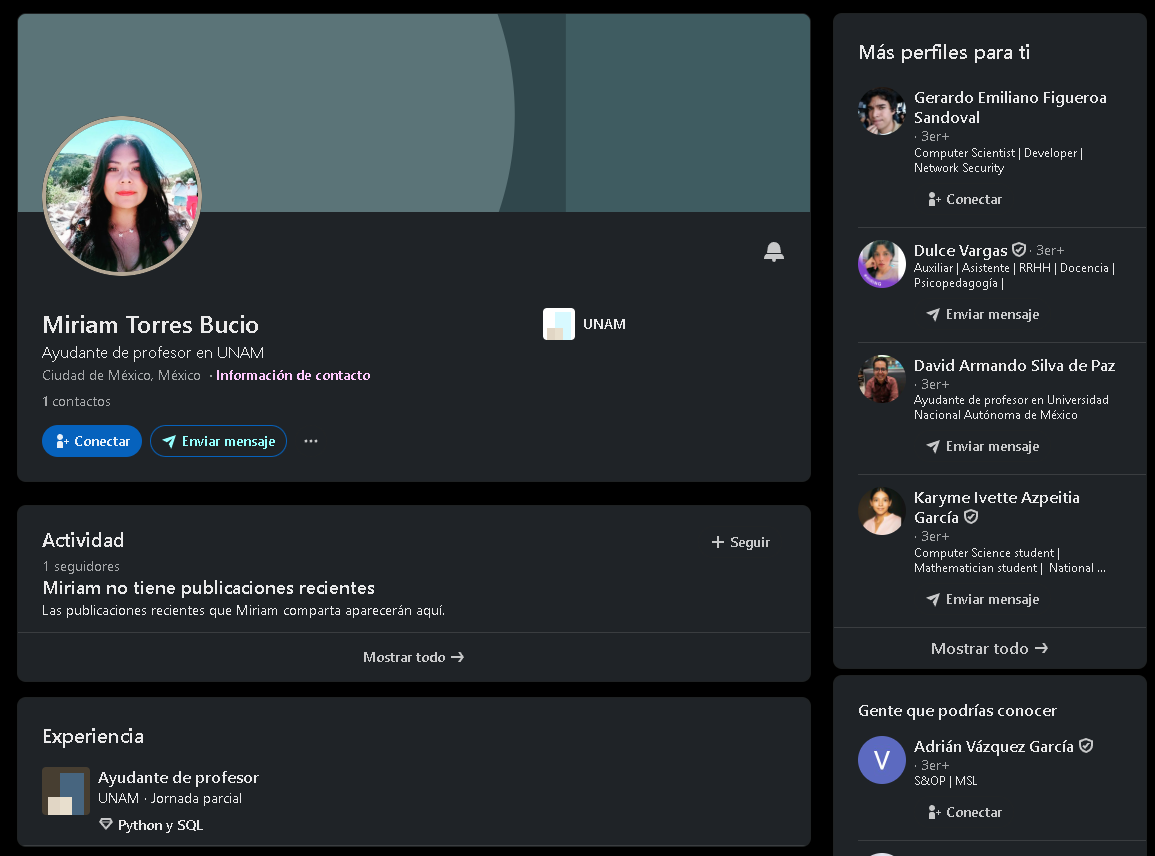
\includegraphics[width=0.45\textwidth]{Imagenes/linkedin1.png}
    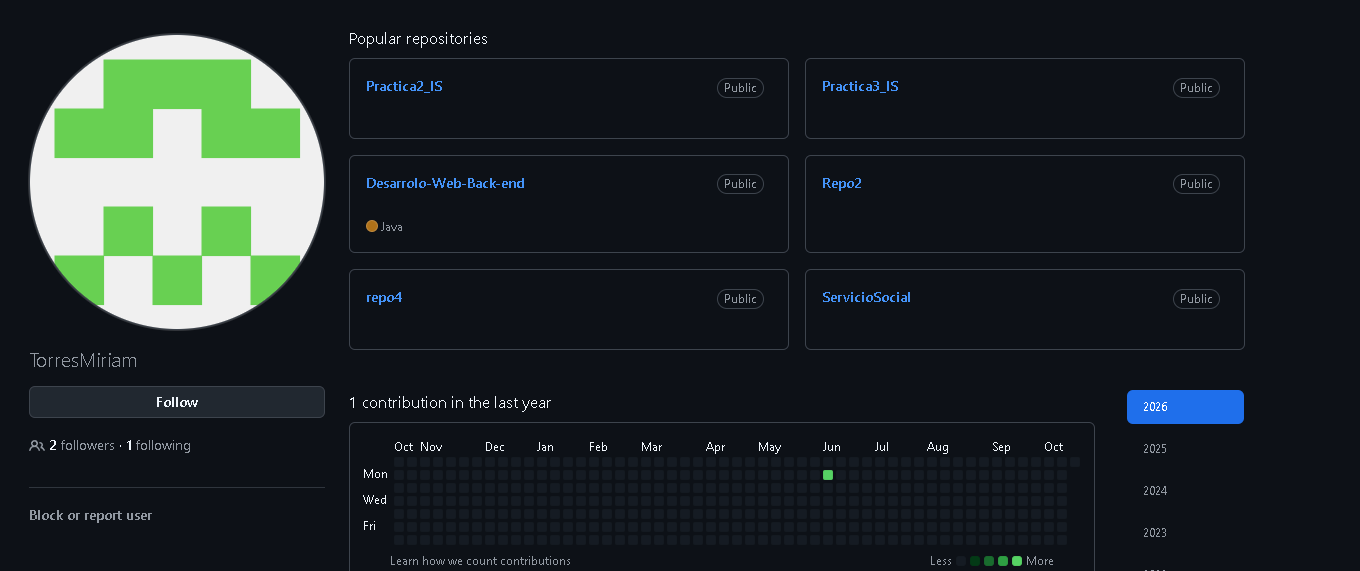
\includegraphics[width=0.45\textwidth]{Imagenes/github1.png}
    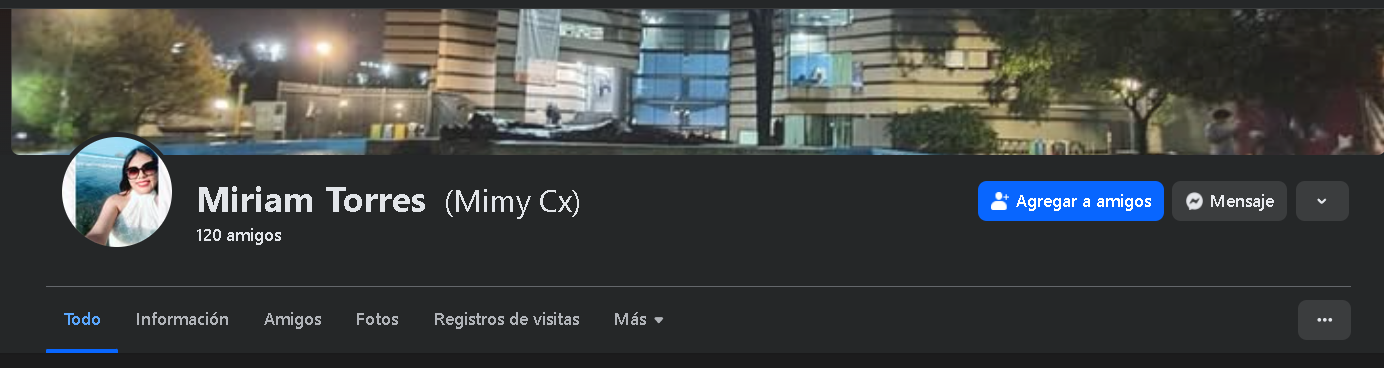
\includegraphics[width=0.45\textwidth]{Imagenes/facebook1.png}
    \caption{Evidencia de perfiles en LinkedIn, GitHub y Facebook.}
\end{figure}

\subsubsection{Información no encontrada}
Con las fuentes revisadas (Google, buscadores internos de redes sociales, LinkedIn, Facebook y GitHub) no logramos localizar información pública suficiente sobre los siguientes puntos:
\begin{itemize}
    \item \textbf{Cumpleaños y edad:} no aparecen en sus perfiles públicos.
    \item \textbf{Familiares y relaciones cercanas:} no se identificaron familiares, pareja ni amigos cercanos de forma confiable.
    \item \textbf{Mascotas:} no se encontraron fotos ni menciones de mascotas.
    \item \textbf{Eventos importantes:} no se hallaron fechas relevantes (graduaciones, viajes, convenciones, etc.) más allá del inicio de su actividad como ayudante.
    \item \textbf{Género musical, color, videojuego y país favorito:} no se encontraron datos públicos que permitan afirmarlos.
\end{itemize}
% TODO: si al revisar el Facebook (fotos, páginas que sigue, eventos) encuentras algo de lo anterior, muévelo a su apartado con su fuente.

\subsubsection{Personalidad}
Con lo recopilado, la agente Miri parece una persona discreta y reservada en internet, con poca actividad pública y un perfil enfocado en lo técnico y lo académico (Python, SQL y docencia). Esta es una inferencia con poca evidencia, justamente porque hay muy poco contenido personal publicado.

\subsubsection{Geolocalización y Análisis de Imágenes}
% TODO: la práctica pide al menos 5 imágenes de lugares no triviales con coordenadas exactas.
% Si encuentras fotos de lugares de Miri, agrégalas con este formato:
% \begin{figure}[H]
%     \centering
%     \includegraphics[width=0.4\textwidth]{Imagenes/miriX.png}
%     \caption{Lugar X. Contexto: ... Coordenadas inferidas: XX.XXXX° N, -XX.XXXX° W. Herramientas: ...}
% \end{figure}
En las cuentas públicas de la agente Miri no se localizaron fotografías de lugares que permitieran determinar coordenadas exactas, por lo que este punto queda como un intento fallido: sus perfiles tienen poco contenido visual y casi toda su información es profesional.

\subsubsection{Herramientas e intentos fallidos}
\begin{itemize}
    \item \textbf{Herramientas:} Google con búsqueda exacta entre comillas, buscadores internos de redes sociales, comparación manual de fotos de perfil.
    \item \textbf{Intentos fallidos:} la búsqueda con el nombre completo no devolvió publicaciones personales, y los perfiles públicos no mostraron datos de familia, mascotas ni eventos.
\end{itemize}

%==========================================================
\subsection{Investigación: Agente Chipotles}

Después de la primera investigación al agente Miri, pasamos a investigar al segundo agente, Chipotles. Inicialmente, realizamos una búsqueda en Google con su nombre completo, usando comillas (\texttt{"Gerardo Emiliano Figueroa Sandoval"}). Encontramos coincidencias en portales profesionales como LinkedIn y en el directorio de la Facultad de Ciencias de la UNAM.

\begin{figure}[H]
    \centering
    
\includegraphics[width=0.6\textwidth]{Imagenes/Busqueda2.png}
    \caption{Búsqueda en Google.}
\end{figure}

Tras agotar los resultados evidentes en los motores de búsqueda convencionales, la investigación pivotó hacia un enfoque de prueba y error manual dentro de los buscadores internos de distintas redes sociales. Fraccionando su nombre y combinando sus apellidos, logramos encontrar su presencia en diversas plataformas digitales. Al cruzar alias recurrentes (como ``Emiliano-FS'' o ``Figue-amigo'') y comparar sus fotografías de perfil, descubrimos sus cuentas personales en plataformas orientadas al entretenimiento y la interacción social, revelando aspectos de su vida personal y profesional.

\subsubsection{Perfil Profesional y Académico}
\begin{itemize}
    \item \textbf{Ocupación:} Se define como Científico de la Computación, Desarrollador y Especialista en Seguridad de Redes.
    \item \textbf{Actividad en la UNAM:} Se desempeña como Ayudante en el área de Ciencias de la Computación desde febrero de 2023. Es egresado en el año 2022.
    \item \textbf{Edad estimada (inferencia):} Basado en un ingreso a la carrera entre 2018 y 2019 y su egreso en 2022, se deduce que tiene una edad aproximada de entre 24 y 27 años. No encontramos su fecha de cumpleaños.
    \item \textbf{Idiomas:} Sabe desenvolverse en inglés y japonés, además de su lengua materna, el español.
    \item \textbf{Correo institucional:} \texttt{efs\_070@ciencias.unam.mx}
\end{itemize}

\subsubsection{Huella Digital y Redes Sociales}
A través del mapeo de su presencia digital, se identificaron los siguientes perfiles públicos:
\begin{itemize}
    \item \textbf{GitHub:} \url{https://github.com/Emiliano-FS}
    \item \textbf{LinkedIn:} \url{https://www.linkedin.com/in/gerardo-emiliano-figueroa-sandoval-3b7849216/}
    \item \textbf{Facebook:} \url{https://www.facebook.com/Felix.McLennon}
    \item \textbf{Instagram:} \url{https://www.instagram.com/dgtal.front___/}
\end{itemize}
Aunque el enlace de Facebook usa un nombre distinto, lo identificamos como suyo por las fotografías de perfil, los alias recurrentes y los contactos en común con sus otras cuentas.

\begin{figure}[H]
    \centering
    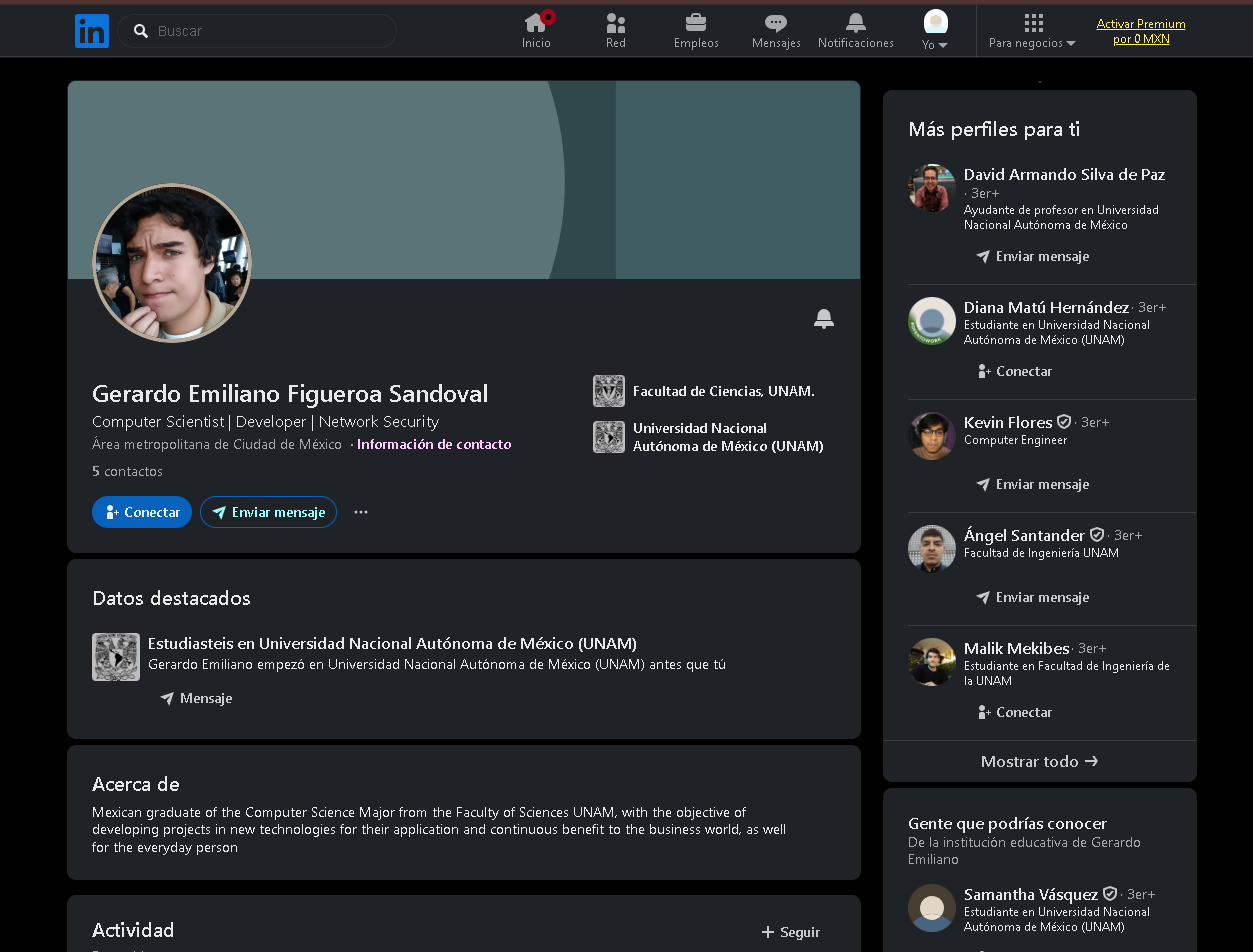
\includegraphics[width=0.45\textwidth]{Imagenes/linkedin2.png}
    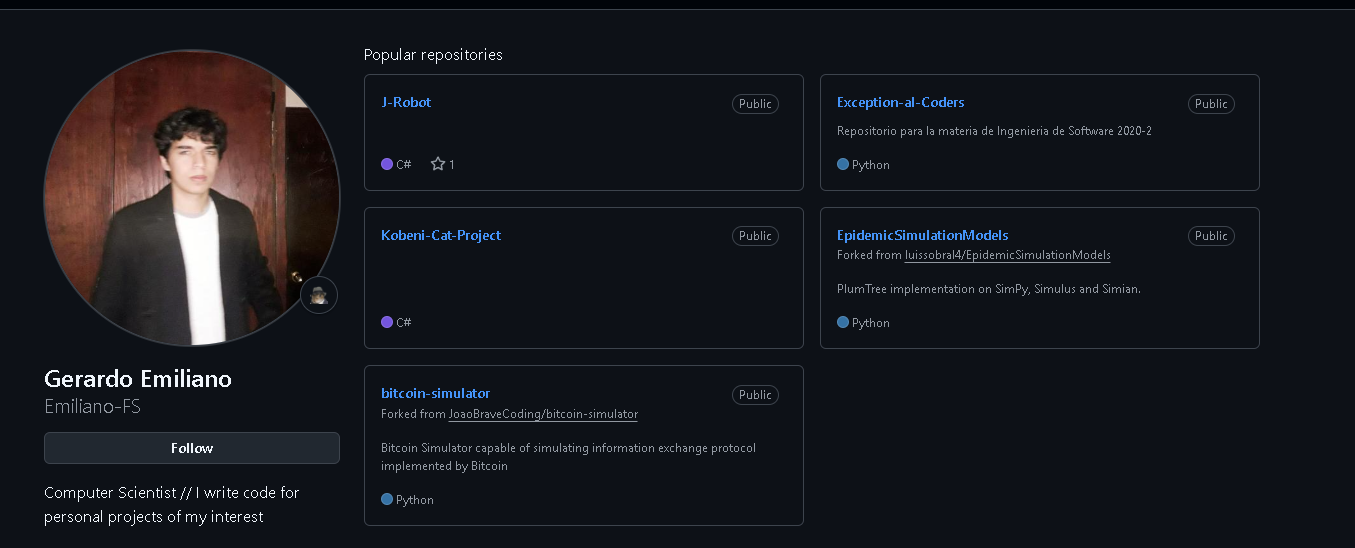
\includegraphics[width=0.45\textwidth]{Imagenes/github2.png}
    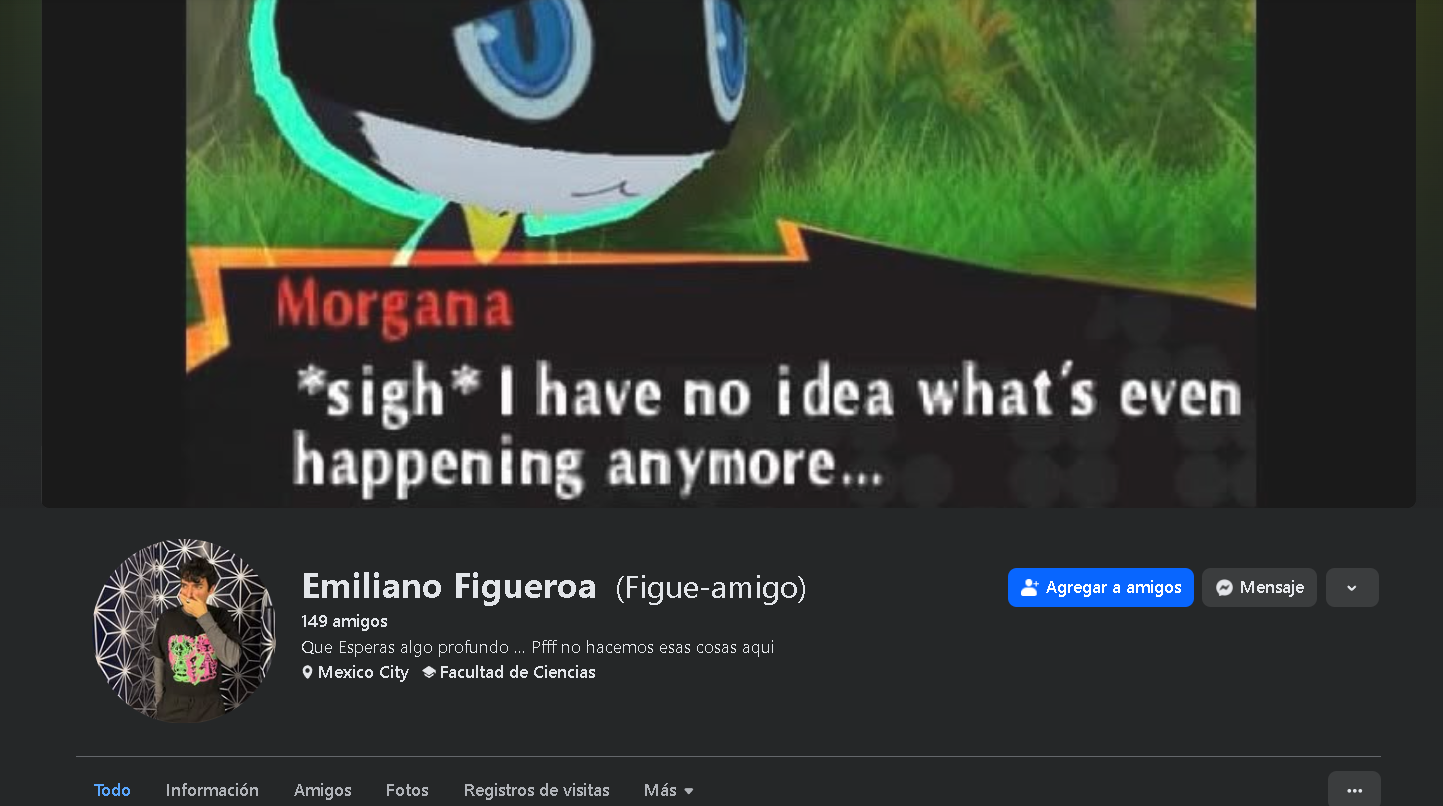
\includegraphics[width=0.45\textwidth]{Imagenes/facebook2.png}
    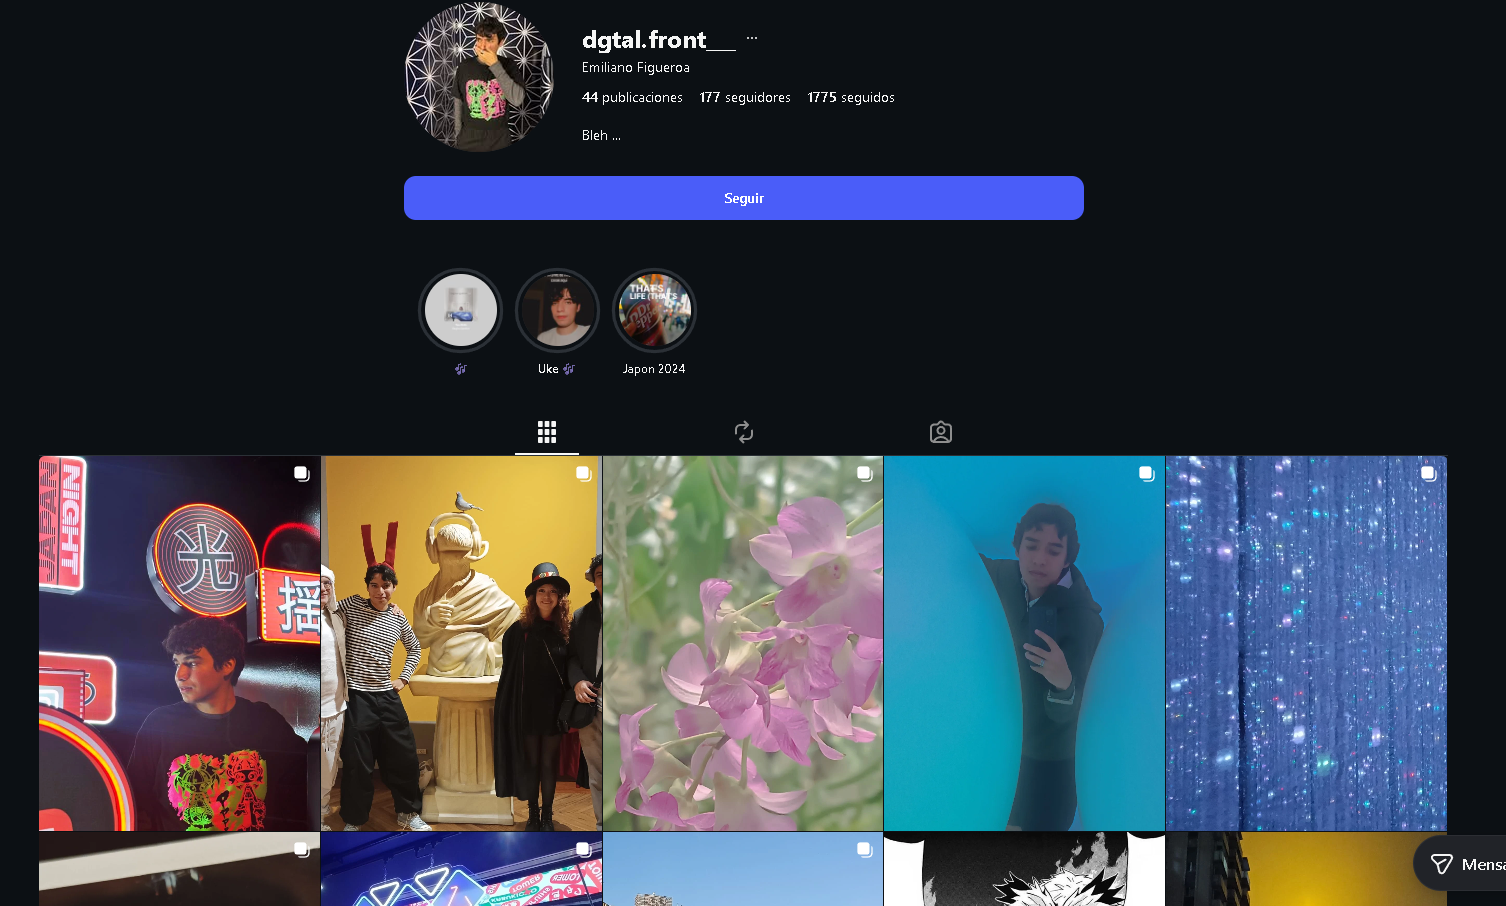
\includegraphics[width=0.45\textwidth]{Imagenes/instagram2.png}
    \caption{Evidencia de perfiles en LinkedIn, GitHub y redes sociales.}
\end{figure}

\subsubsection{Aspectos Personales y Personalidad}
Al analizar las publicaciones e interacciones en sus redes personales (Facebook e Instagram), se perfiló la siguiente información:
\begin{itemize}
    \item \textbf{Cultura y viajes:} Se observa una afinidad por Japón y su cultura, pues cuenta con fotos de sus viajes.
    \item \textbf{Entretenimiento:} Consume anime y manga, destacando \textit{Evangelion} y \textit{Boku no Hero}. También disfruta de videojuegos como \textit{Persona 5} (que aparece en la portada de su perfil de Facebook) y de la serie \textit{31 Minutos} (fue a la exposición presentada en CDMX).
    \item \textbf{Hobbies:} Se le observa tocando el ukulele. También se ha disfrazado de diversos personajes para eventos de Halloween o convenciones de anime y cómic.
    \item \textbf{Círculo cercano:} Se observan interacciones frecuentes que denotan amistad con los usuarios de Instagram \texttt{bere.borrego} y \texttt{angel\_g\_g580}, que podrían ser amigos cercanos suyos.
\end{itemize}

Algunos eventos o fechas importantes que encontramos en sus redes sociales fueron:
\begin{itemize}
    \item \textbf{Graduación:} Se graduó en 2022, pues el 31 de mayo subió una foto con su toga y birrete.
    \item \textbf{Exposición de 31 Minutos:} Fue a la exposición en CDMX que se presentó durante el último trimestre de 2024 y hasta mediados de enero de 2025. Fue acompañado de sus amigos.
    \item \textbf{Viaje a Japón:} Se le observa en fotos de su viaje a Japón, aproximadamente en 2024.
\end{itemize}

Al recabar esta información, podemos deducir algunas características de su personalidad, como su sentido del humor, su gusto por la cultura japonesa y su interés en la seguridad informática. También podemos inferir que es una persona sociable, con un círculo cercano de amigos y que disfruta de actividades culturales y de entretenimiento.

Durante la revisión de su muro público de Facebook, se localizó un bloque de texto codificado en formato hexadecimal, dejado a manera de reto o broma para quienes revisan su perfil:

\begin{quote}
% OJO: verifica que esta cadena esté copiada exactamente igual que en su publicación original.
\texttt{4372656f207175652061636162617320646520676173746172207475207469656d706f20656e20\\
6573746f203a702021a536f6e7269652061206c612063e16d61726120212026486168616861686\\
12045726573206D757920636F6F6C202026}
\end{quote}

Al procesar esta cadena mediante un decodificador de hexadecimal a ASCII, se obtuvo el siguiente mensaje en texto plano:
\begin{quote}
\textit{``Creo que acabas de gastar tu tiempo en esto :p ! sonríe a la cámara ! Hahahahaha Eres Muy cOoL''}
\end{quote}
Esto muestra su gusto por los retos de codificación y cómo integra la seguridad informática a su sentido del humor.

\subsubsection{Gustos y preferencias}
\begin{itemize}
    \item \textbf{Videojuegos:} Disfruta de los videojuegos, aunque no podemos determinar con certeza su título favorito (podría ser \textit{Persona 5}).
    \item \textbf{País favorito:} Inferimos que es Japón, pues tomó muchas fotos de su viaje allá.
    \item \textbf{Música:} Algunos de sus gustos son artistas como \textit{Jósean Log} y \textit{Metric}, y música japonesa.
    \item \textbf{Color favorito, mascotas y familia:} No pudimos determinarlos. No hay fotos de mascotas en sus redes ni información de su familia.
\end{itemize}

\subsubsection{Geolocalización y Análisis de Imágenes}

Originalmente se planteó utilizar la herramienta \texttt{exiftool} para extraer los metadatos de ubicación incrustados en las fotografías. Sin embargo, dado que todas las imágenes recopiladas de este objetivo provienen de plataformas de redes sociales (Instagram y Facebook), esta vía fue descartada. Estas plataformas aplican un proceso automático de limpieza de metadatos al momento de subir los archivos, eliminando etiquetas como \texttt{GPSLatitude} y \texttt{GPSLongitude} por motivos de privacidad.

En su lugar, se emplearon técnicas de Inteligencia Geoespacial (GEOINT) y de observación visual. Mediante la observación de elementos arquitectónicos, puntos de referencia y el contexto de sus publicaciones, se lograron inferir las ubicaciones de las siguientes 5 fotografías.

\begin{figure}[H]
    \centering
    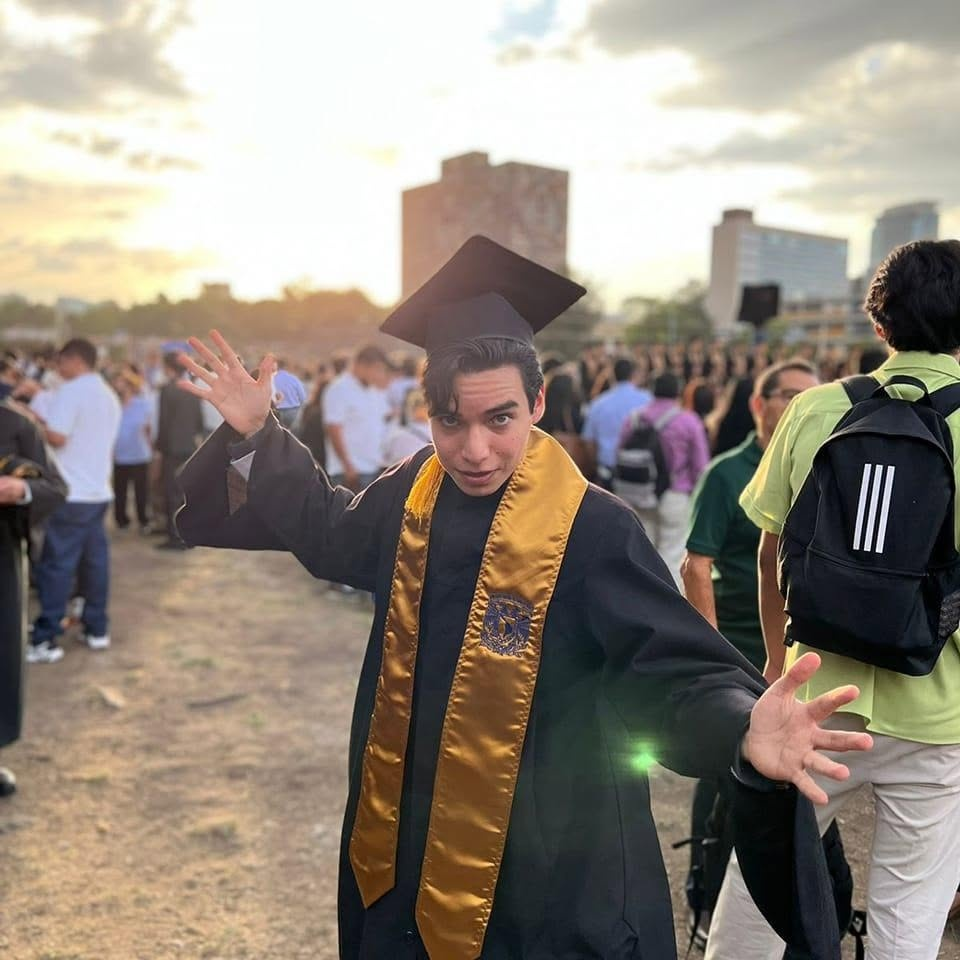
\includegraphics[width=0.35\textwidth]{Imagenes/unam.png}
    \caption{Lugar 1. Contexto: Fotografía de graduación en ``Las Islas'' de Ciudad Universitaria, UNAM. Al fondo se observa la Torre de Rectoría. Coordenadas inferidas: 19.3315° N, -99.1868° W.}
\end{figure}

\begin{figure}[H]
    \centering
    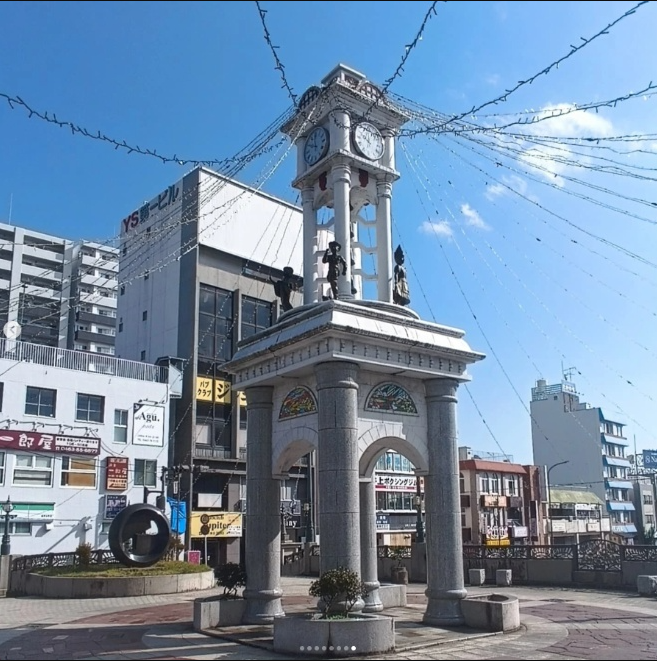
\includegraphics[width=0.35\textwidth]{Imagenes/reloj.png}
    \caption{Lugar 2. Contexto: Torre del Reloj autómata del Puente Mahoroba, Japón. Identificado mediante reconocimiento de arquitectura turística asiática. Coordenadas inferidas: 35.37433° N, 139.22658° E.}
\end{figure}

\begin{figure}[H]
    \centering
    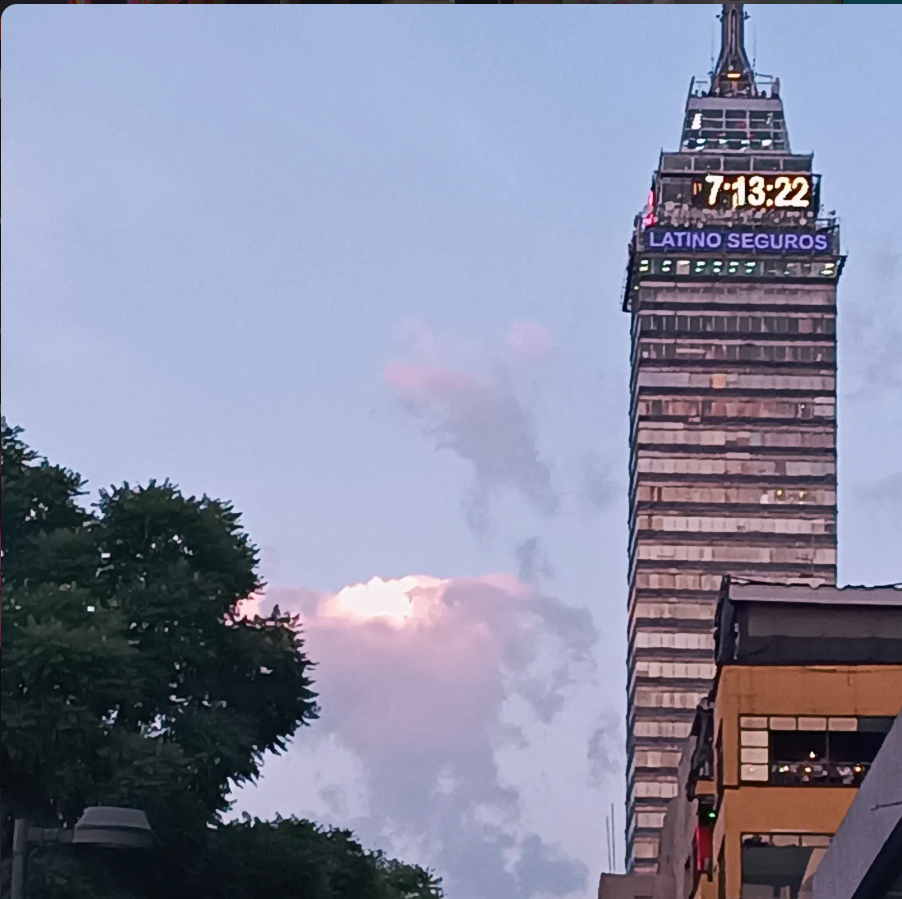
\includegraphics[width=0.35\textwidth]{Imagenes/torre.png}
    \caption{Lugar 3. Contexto: Torre Latinoamericana, Ciudad de México. Fotografía tomada desde el nivel de calle en las inmediaciones del Centro Histórico. Coordenadas inferidas: 19.4339° N, -99.1405° W.}
\end{figure}

\begin{figure}[H]
    \centering
    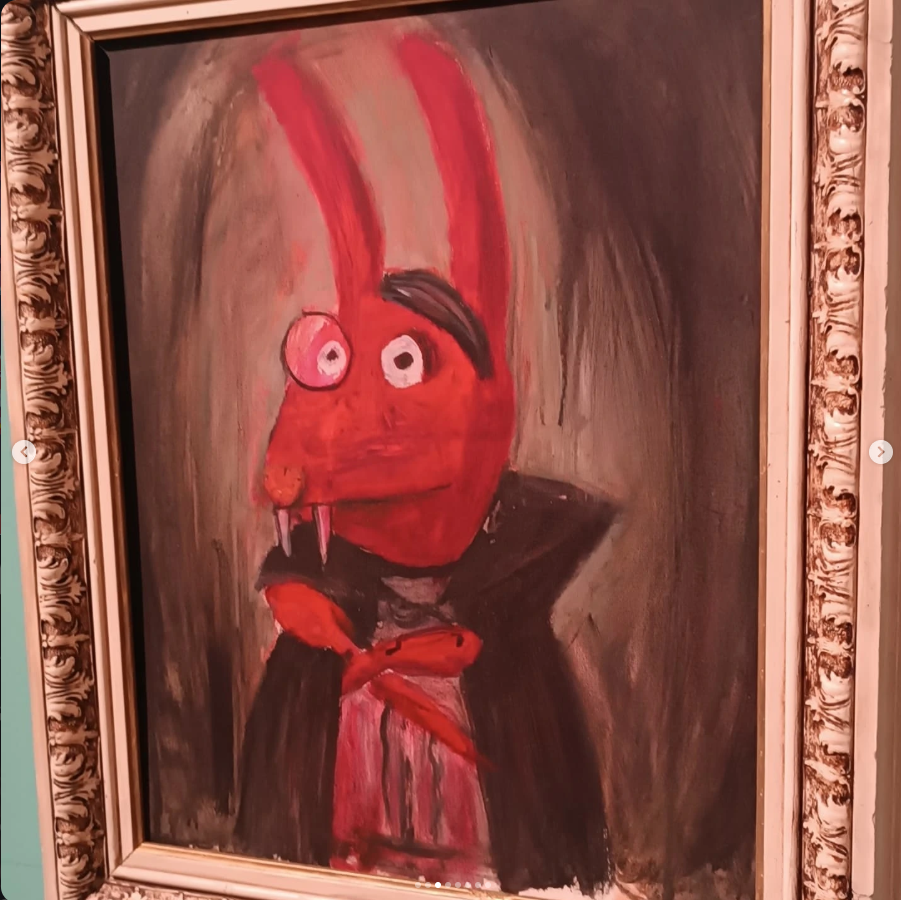
\includegraphics[width=0.35\textwidth]{Imagenes/museo.png}
    \caption{Lugar 4. Contexto: Pintura expuesta en el ``Museo 31'' (Exposición de 31 Minutos), que tuvo lugar en el Museo Franz Mayer en la Ciudad de México. Coordenadas inferidas: 19.4373° N, -99.1434° W.}
\end{figure}

\begin{figure}[H]
    \centering
    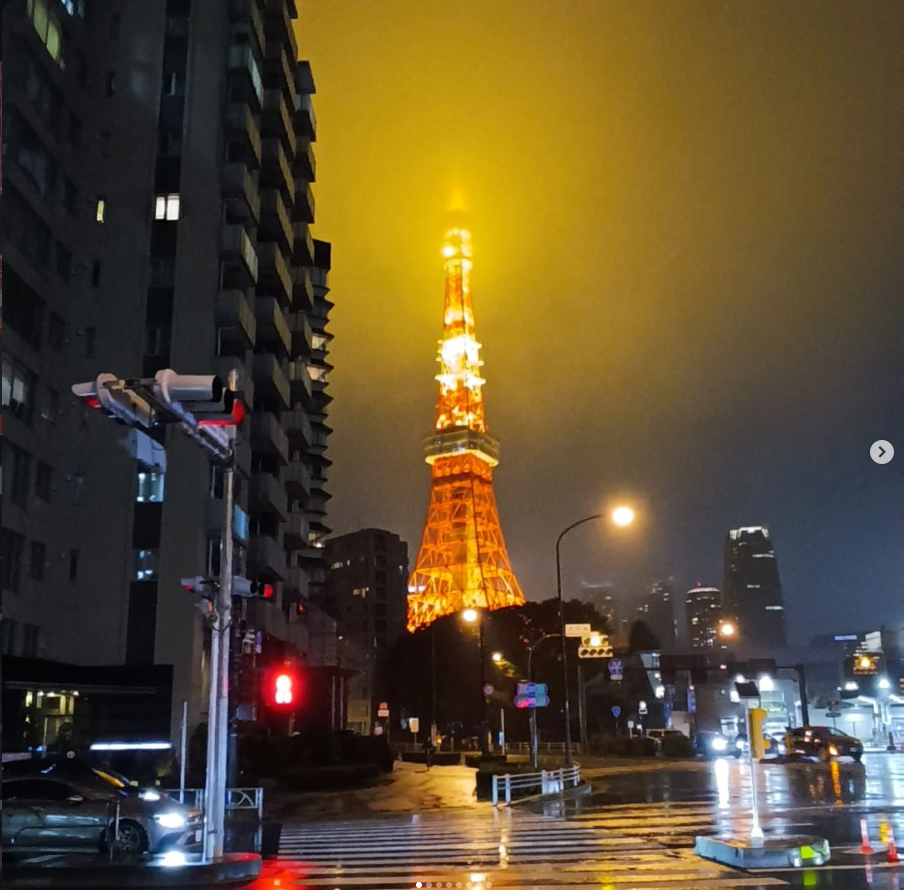
\includegraphics[width=0.35\textwidth]{Imagenes/tokio.png}
    \caption{Lugar 5. Contexto: Torre de Tokio (Tokyo Tower) en Minato City, Japón. La ubicación fue confirmada tanto visualmente como por la etiqueta de geolocalización directa en su publicación. Coordenadas inferidas: 35.6585° N, 139.7454° E.}
\end{figure}

\subsubsection{Herramientas e intentos fallidos}
\begin{itemize}
    \item \textbf{Herramientas:} Google con búsqueda exacta entre comillas, buscadores internos de redes sociales, comparación manual de fotos de perfil, decodificador hexadecimal a ASCII, Google Maps y Street View para confirmar ubicaciones.
    \item \textbf{Intentos fallidos:} \texttt{exiftool} no sirvió porque las redes sociales eliminan los metadatos; no se hallaron mascotas, familiares ni color favorito en sus perfiles públicos.
\end{itemize}

\clearpage
